\section{Foresta dei Giganti}\label{foresta-dei-giganti}

Tags: Luogo di interesse Creatore: Davide, Lorenzo

\section{Foresta dei Giganti}\label{foresta-dei-giganti-1}

\begin{center}\rule{0.5\linewidth}{0.5pt}\end{center}

\begin{figure}
\centering
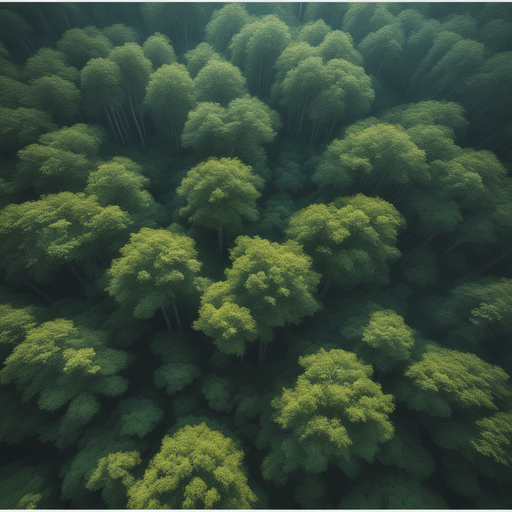
\includegraphics{imagine-a-breathtaking-aerial-view-of-the-mystical-forest-from-above-the-towering-ancient-trees-st-3.png}
\caption{imagine-a-breathtaking-aerial-view-of-the-mystical-forest-from-above-the-towering-ancient-trees-st-3.png}
\end{figure}

Informazioni Generali

Tipo di Luogo:

Dimensioni:

Altitudine:

Popolazione:

Paese:

Luogo:

Alleata con:

Attività:

\begin{center}\rule{0.5\linewidth}{0.5pt}\end{center}

\subsection{1. Descrizione Generale}\label{descrizione-generale}

\begin{center}\rule{0.5\linewidth}{0.5pt}\end{center}

\begin{figure}
\centering
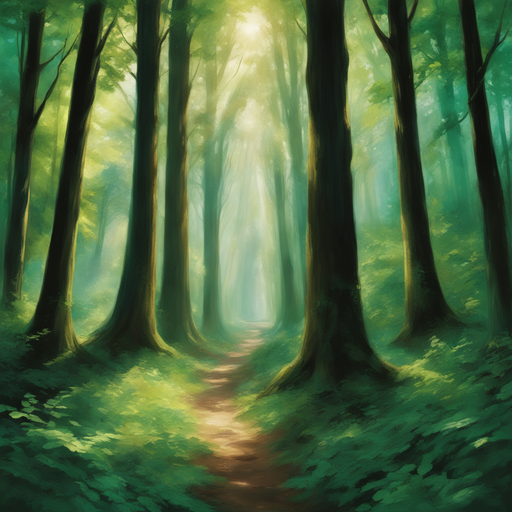
\includegraphics{picture-yourself-standing-within-the-heart-of-the-forest-surrounded-by-towering-trees-their-branch.png}
\caption{picture-yourself-standing-within-the-heart-of-the-forest-surrounded-by-towering-trees-their-branch.png}
\end{figure}

La Foresta dei Giganti, situata al cuore della regione di Valtara, è un
gioiello naturale che cattura l'immaginazione di chiunque vi ponga lo
sguardo. Questo vasto bosco è caratterizzato da alberi maestosi che si
innalzano alto sopra gli altri, creando una volta naturale che offre
spettacolari scenari di verde e uno straordinario senso di meraviglia.
Il paesaggio presenta colline dolci e montagne imponenti, mentre il
fiume Kratos, il principale corso d'acqua della regione, serpeggia
attraverso la foresta, contribuendo alla sua bellezza senza tempo.

\subsection{2. Storia}\label{storia}

\begin{center}\rule{0.5\linewidth}{0.5pt}\end{center}

La storia della Foresta dei Giganti risale a tempi antichi, quando
veniva considerata una terra sacra dalle tribù indigene della regione di
Valtara. Queste tribù, che un tempo abitavano i boschi e le colline,
veneravano gli alberi secolari come guardiani spirituali e facevano
cerimonie rituali per onorare la natura selvaggia.

Con il passare dei secoli, la foresta ha assistito a molte
vicissitudini, diventando teatro di avventure, esplorazioni e leggende.
Si racconta che antiche rovine nascoste tra gli alberi siano il rifugio
di spiriti ancestralii e guardiani delle profondità della foresta.
Queste rovine sono state oggetto di numerose spedizioni, ma solo pochi
coraggiosi sono tornati per raccontare le loro esperienze.

\subsection{3. Geografia}\label{geografia}

\begin{center}\rule{0.5\linewidth}{0.5pt}\end{center}

La Foresta dei Giganti occupa un'area collinare e montuosa, offrendo una
varietà di paesaggi mozzafiato. Tra gli alberi altissimi, tra cui querce
secolari e maestosi abeti, i visitatori possono trovare rifugio
dall'ardente sole estivo. Il suolo è ricoperto da una vasta gamma di
piante, muschi e felci, creando un tappeto verde che si estende fino
all'orizzonte.

Al centro della foresta scorre il fiume Kratos, il cui percorso sinuoso
attraverso il bosco crea una scenografia di rara bellezza. Questo fiume
è il principale punto di approvvigionamento d'acqua per la regione di
Valtara, rendendo la foresta cruciale per l'ecosistema locale

\subsection{4. Flora e Fauna}\label{flora-e-fauna}

\begin{center}\rule{0.5\linewidth}{0.5pt}\end{center}

La Foresta dei Giganti è un'esplosione di vita, con una varietà di flora
e fauna che la abita. Gli alberi giganteschi, tra cui querce secolari,
abeti maestosi e pioppi possenti, dominano il paesaggio. Man mano che ci
si avvicina al centro della foresta, gli alberi diventano sempre più
imponenti, con alcuni che raggiungono altezze straordinarie, tanto da
scomparire tra le nuvole. Questi alberi giganti sono le colonne portanti
della foresta, contribuendo a creare un'atmosfera maestosa e misteriosa.

La fauna è altrettanto affascinante. Si possono avvistare cervi maestosi
che si librano tra gli alberi, lepri veloci che sfrecciano attraverso il
sottobosco e lupi solitari che scrutano dalla penombra. Tuttavia, più ci
si avventura verso il centro della foresta, più gli animali diventano
selvaggi e misteriosi. Si racconta di creature leggendarie e magici
abitanti della foresta, che fanno parte delle leggende e delle storie
tramandate di generazione in generazione.

Varie leggende raccontano di come al centro di tutto ciò si erga
l'Albero Colossale, la corona della flora nella foresta. Si dice che
questo albero possieda poteri magici e abbia una connessione profonda
con la natura stessa. La sua immagine maestosa e la sua aura misteriosa
rappresentano il cuore pulsante della Foresta dei Giganti e la sua
eredità millenaria

\subsection{5. Persone famose}\label{persone-famose}

\begin{center}\rule{0.5\linewidth}{0.5pt}\end{center}

Tra i personaggi famosi associati alla Foresta dei Giganti spicca Elara
Ventoscura, una druida rispettata per la sua conoscenza delle erbe
medicinali e delle creature della foresta. Elara è considerata una
custode della foresta e ha dedicato la sua vita a proteggerla e a
promuovere la sua conservazione.

Inoltre, il cacciatore leggendario Garret Lupo Nero è noto per le sue
avventure nelle profondità della foresta alla ricerca di creature
mitiche e pericolose. Le sue storie di incontri con creature leggendarie
hanno ispirato numerosi avventurieri a esplorare la foresta e a cercare
di catturare la sua essenza misteriosa.

\subsection{A. Galleria Immagini}\label{a.-galleria-immagini}

\begin{figure}
\centering
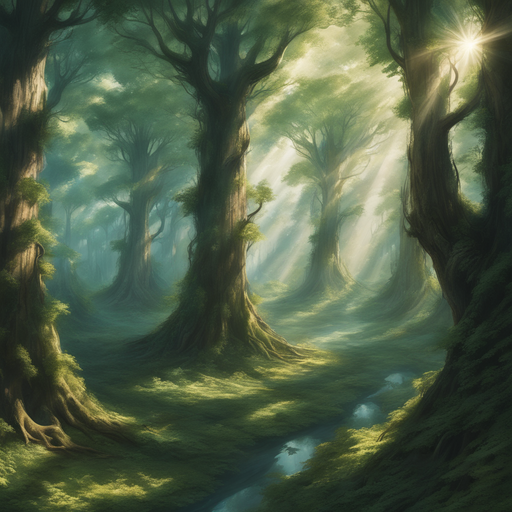
\includegraphics{imagine-a-breathtaking-aerial-view-of-the-mystical-forest-from-above-the-towering-ancient-trees-st-4.png}
\caption{imagine-a-breathtaking-aerial-view-of-the-mystical-forest-from-above-the-towering-ancient-trees-st-4.png}
\end{figure}

\begin{figure}
\centering
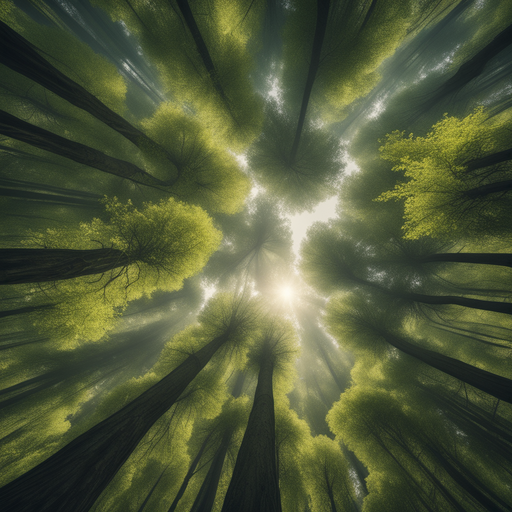
\includegraphics{imagine-a-breathtaking-aerial-view-of-the-mystical-forest-from-above-the-towering-ancient-trees-st.png}
\caption{imagine-a-breathtaking-aerial-view-of-the-mystical-forest-from-above-the-towering-ancient-trees-st.png}
\end{figure}

\begin{figure}
\centering
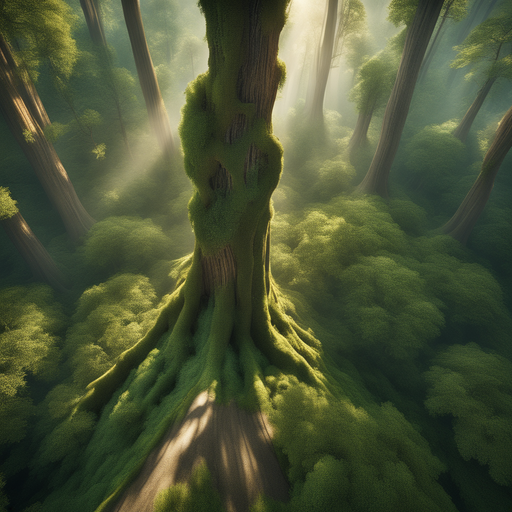
\includegraphics{imagine-a-breathtaking-aerial-view-of-the-mystical-forest-from-above-the-towering-ancient-trees-st-2.png}
\caption{imagine-a-breathtaking-aerial-view-of-the-mystical-forest-from-above-the-towering-ancient-trees-st-2.png}
\end{figure}
